%\chapter{Implémentation}
%
%%%%%%%%%%%%%%%%%%%%%%%%%%%%%%%%%%%%%%%%%%%%%%%%%%%%%%%%%%%%%%%%%%%%%%%%%%%%%%%%
%\section{Limitations}
%        Le driver Wi-Fi d'\textit{IDF} ne nous permet pas d'avoir une connexion
%        avec plusieurs noeuds simultanément. \espnow\ pourraît être une solution
%        pour palier à ce problème.\\
%    
%    
%        \textbf{ESP NOW}\\
%            \espnow\ est un protocole de communication Wi-Fi sans connexion défini
%            par Espressif.\\ Nous n'avons trouvé aucune documentation décrivant le
%            fonctionnement de ce protocole.\\
%            Avec la documentation disponible, nous savons qu'un noeud a une liste
%            de \textit{peers} (ses voisins) avec qui il peut échanger des données.
%            Le nombre de voisins est limité à 20. Cette limite ne posera pas 
%            problème pour ce projet.
%        
%%%%%%%%%%%%%%%%%%%%%%%%%%%%%%%%%%%%%%%%%%%%%%%%%%%%%%%%%%%%%%%%%%%%%%%%%%%%%%%%
%\section{Prochaines étapes}
%        \begin{enumerate}
%            \item Nous allons créer un réseau \espmesh. Ceci nous permettra de nous
%            familiariser avec l'environnement \textit{IDF}.
%            \item Nous évaluerons les performances et fonctionnalités de ce protocole.
%            \item Nous implémenterons un protocole de routage mesh choisis plus haut.
%            \item L'objectif est de l'implémenter au niveau de la couche liaison de données.
%                Si nous rencontrons trop de difficulté ou que nous jugeons que ce 
%                choix n'est pas judicieux, nous implémenterons ce protocole au niveau 
%                de la couche réseau.
%            \item Nous étudierons les différentes possibilités d'économies d'énergie
%            \item Nous évaluerons les performances et fonctionnalités du prorotype créé. 
%            
%        \end{enumerate}

\chapter{Mise en oeuvre}
    \todo{INTRO}\\
    Nous avons utilisé la version 3.3.1 d'IDF car c'est une version stable suportée jusqu'en février 2022.
    \section{ESP-MESH}
    %\begin{enumerate}
        %\item \textbf{\underline{Construction du réseau}}\\
        \textbf{\underline{Construction du réseau}}\\
            Notre première étape a été d'établir un réseau \espmesh\ composé de deux noeuds (une racine et son enfant).
            Voici un extrait du code permettant de construire ce réseau:
            \begin{minted}[xleftmargin=\parindent,linenos]{c}
void app_main(void){
    /* stop DHCP server for softAP and station interfaces */
    ESP_ERROR_CHECK(tcpip_adapter_dhcps_stop(TCPIP_ADAPTER_IF_AP));
    ESP_ERROR_CHECK(tcpip_adapter_dhcpc_stop(TCPIP_ADAPTER_IF_STA));
    /* wifi initialisation */ 
    wifi_init_config_t config = WIFI_INIT_CONFIG_DEFAULT();
    ESP_ERROR_CHECK(esp_wifi_init(&config));
    ESP_ERROR_CHECK(esp_wifi_start());
    /*  mesh initialisation*/
    ESP_ERROR_CHECK(esp_mesh_init());
    mesh_cfg_t cfg = MESH_INIT_CONFIG_DEFAULT();
    /* event handler */
    cfg.event_cb = &mesh_event_handler;
    /* ... */
    ESP_ERROR_CHECK(esp_mesh_set_config(&cfg)); //set mesh configuration
    ESP_ERROR_CHECK(esp_mesh_start()); //start mesh network
}
            \end{minted}
            On remarque que nous désactivons le serveur DHCP. En effet, la racine étant la passerelle entre 
            le réseau \espmesh\ et l'extérieur, elle est la seule à avoir besoin d'une adresse \textsc{ip}.
            Le serveur DHCP sera activé sur la racine une fois celle-ci élue.
            Ensuite le \wifi\ est initialisé ainsi que le réseau \espmesh, pour enfin démarrer ce dernier.\\
            
            
            Analysons maintenant la construction du réseau avec deux noeuds. Tout d'abord, 
            considérer les logs d'un \esp. Ensuite nous passerons à l'analyse des communications obtenue
            avec Wireshark.\footnote{les logs et la trace Wireshark ont été réduit pour ne garder 
            que les données utiles à la compréhension du fonctionnement d'un réseau \espmesh.}
            \begin{minted}[xleftmargin=\parindent,linenos]{console}
I (1479) mesh: <MESH_NWK_LOOK_FOR_NETWORK>need_scan:0x1, 
    need_scan_router:0x0, look_for_nwk_count:1
I (1779) mesh: [FIND][ch:7]AP:0, otherID:0, MAP:0, idle:0, 
    candidate:0, root:0[00:00:00:00:00:00]
I (1779) mesh: [FIND:1]fail to find a network, channel:0, 
    cfg<channel:7, router:MyRouter, 00:00:00:00:00:00>

I (1789) mesh: <MESH_NWK_LOOK_FOR_NETWORK>need_scan:0x3, 
    need_scan_router:0x1, look_for_nwk_count:2
I (1919) mesh: [S1]MyRouter, 1a:b2:c3:d4:e5:f6, channel:7, rssi:-43
I (1919) mesh: find router:[ssid_len:13]MyRouter, rssi:-43, 
    1a:b2:c3:d4:e5:f6(encrypted), new channel:7, old channel:0
I (1929) mesh: [FIND][ch:7]AP:1, otherID:0, MAP:0, idle:0, candidate:0, 
    root:0[1a:b2:c3:d4:e5:f6]router found<scan router>
I (1939) mesh: [FIND:2]find a network, channel:7, cfg<channel:7, 
    router:MyRouter, 00:00:00:00:00:00>

I (1949) wifi: mode : sta (3c:71:bf:0d:83:08) + softAP (3c:71:bf:0d:83:09)
I (2269) mesh: [SCAN][ch:7]AP:2, other(ID:0, RD:0), MAP:1, idle:1,
    candidate:1,root:0, topMAP:0[c:1,i:1][1a:b2:c3:d4:e5:f6]router found<>
I (2269) mesh: 1022<pre>my_vote_num:0, voter_num/max_connection:4,
    2nd_layer_count:0
I (2279) mesh: 6104[SCAN]init rc[ttl:127/votes:1][3c:71:bf:0d:7e:1d,-120]
I (2279) mesh: 6104[SCAN]init rc[ttl:127/votes:1][3c:71:bf:0d:7e:1d,-120]
I (2289) mesh: 1250, vote myself, router rssi:-45 > voted rc_rssi:-120
I (2299) mesh: [SCAN:1/10]rc[128][3c:71:bf:0d:83:09,-45], 
    self[3c:71:bf:0d:83:08, -45,reason:0,votes:1,idle]
        [mine:1,voter:1(1.00)percent:0.90][128,1,3c:71:bf:0d:83:09]

                            ....
I (8049) mesh: [SCAN:10/10]rc[128][3c:71:bf:0d:83:09,-45], 
    self[3c:71:bf:0d:83:08,-39,reason:0,votes:2,idle][mine:2,voter:2(1.00)percent:0.90][128,2,3c:71:bf:0d:83:09]

I (8069) mesh: [DONE]connect to router:MyRouter, channel:7,
    rssi:-39, 1a:b2:c3:d4:e5:f6[layer:0, assoc:0], my_vote_num:2/voter_num:2, rc[3c:71:bf:0d:83:09/-45/1]
                            
%            \end{minted}

            Nous observons d'abord que le noeud cherche un réseau \espmesh. Comme il n'en trouve pas,
            il cherche un point d'accès. Il trouve le point d'accès \textit{"MyRouter"} qui est sur 
            le canal 7 et avec lequel il a un \rssi\ de -43. En écoutant les beacons
            des autres noeuds, nous remarquons bien qu'il détecte un autre noeud idle.


            Ensuite le vote commence à la ligne 19. À chaque itération du vote, le noeud
            écoute les beacons des autres noeuds, ce qui lui permet de détecter autre noeud idle qui a un \rssi
            avec le routeur de -120. Comme $-45 > -120$, il va voter pour lui-même. C'est à dire, émettre
            un beacon avec ses propres informations. Si son \rssi\ était moins fort que celui de l'autre noeud, 
            il aurait émis un beacon avec les informations de l'autre noeud. Ce que nous avons décrit ici
            correspond à une itération du vote. Dans notre cas il y aura 10 itérations. Ce nombre est un paramètre
            tu réseau \espmesh. A la fin des 10 itérations, le noeud compare son ratio à un seuil prédéfini (ici de 0.90).
            Comme ce ratio (ici de 1) est plus grand que le seuil, le noeud devient la racine du réseau \espmesh\ et 
            se connecte au routeur.
            Ses observations correspondent bien à la description du protocole faite plus haut.
            Concentrons nous maintenant sur les trames capturées avec Wireshark.

            \begin{figure}[H]
                \begin{tikzpicture}
                    \FLOWPART{diagram.tex}{1}{9}
                \end{tikzpicture}
                \caption{Diagramme de séquence des paquets précédent le vote}
            \end{figure}

            Sur la figure ci-dessus, nous observons d'abord deux requêtes \textsc{arp} de la part de chaque \esp\ pour l'adresse
            192.168.4.1 . Nous ignorons la raison de cette requête. Cette adresse \textsc{ip} été associée à un point d'accès
            qui servait également de serveur pour nos premières expérimentations réalisée pour la communication avec une adresse
            externe au réseau \espmesh. Ensuites, nous observons une série de trames de désassociation et désauthentification.
            Après cette étape, le vote d'élection de la racine débute.
            \begin{figure}[H]
                \begin{tikzpicture}
                    \FLOWPART{diagram.tex}{10}{15}
                \end{tikzpicture}
                \caption{Diagramme de séquence d'une itération du vote}        
            \end{figure}
            Nous illustrons sur la figure ci-dessus, une itération de processus de vote.
            Chaque noeud émet d'abord une \textit{Probe Request} pour le point d'accès configuré. Il reçoit ensuite
            une \textit{Probe Request} si le point d'accès est à sa portée. Avec la réception de cette trame,
            le noeud possède les informations dont il a besoin pour émettre son beacon contenant notamment
            sont \textsc{rssi} avec le point d'accès et l'\textsc{id} du réseau \espmesh. Les autres noeuds
            à portée de ce noeud vont recevoir ce beacon et pourront donc voter. Voici un exemple
            d'un beacon émis lors du processus de vote.
            \begin{alltt}
IEEE 802.11 Beacon frame, Flags: ........C
    Type/Subtype: Beacon frame (0x0008)
    Frame Control Field: 0x8000
        .... ..00 = Version: 0
        .... 00.. = Type: Management frame (0)
        1000 .... = Subtype: 8
    Receiver address: Broadcast (ff:ff:ff:ff:ff:ff)
    Destination address: Broadcast (ff:ff:ff:ff:ff:ff)
    Transmitter address: Espressi_0d:83:09 (3c:71:bf:0d:83:09)
    Source address: Espressi_0d:83:09 (3c:71:bf:0d:83:09)
    BSS Id: Espressi_0d:83:09 (3c:71:bf:0d:83:09)
IEEE 802.11 wireless LAN
    Tagged parameters (235 bytes)
        Tag: Vendor Specific: Espressif Inc.
            Tag Number: Vendor Specific (221)
            Tag length: 69
            OUI: 18:fe:34 (Espressif Inc.)
            Vendor Specific OUI Type: 1
            Vendor Specific Data: 010200777777777777190004000000000000
                000000000088880000000000000088000000000000880000000000
                000000000000000000000a0000000f00005f8ad240
        Tag: Vendor Specific: Espressif Inc.
            Tag Number: Vendor Specific (221)
            Tag length: 22
            OUI: 18:fe:34 (Espressif Inc.)
            Vendor Specific OUI Type: 6
            Vendor Specific Data: 0602000b4553504d5f304438333038cd20f923
        Tag: Vendor Specific: Espressif Inc.
            Tag Number: Vendor Specific (221)
            Tag length: 21
            OUI: 18:fe:34 (Espressif Inc.)
            Vendor Specific OUI Type: 12
            Vendor Specific Data: 0c020000000000006defa84d995c80b0d2d3
            \end{alltt}
            Une fois que toutes les itérations ont été réalisées, la racine se connecte au routeur et le deuxième noeud
            se connecte à la racine. Ceci est illustré sur la figure suivante.
            \begin{figure}[H]
                \begin{tikzpicture}
                    \FLOWPART{diagram.tex}{49}{71}
                \end{tikzpicture}
                \caption{Diagramme de séquence des connexions}         
            \end{figure}
            
            Nous remarquons qu'entre les messages 49 et 67, la racine élue se connecte au routeur, et des beacons continue
            à être émis.
            Ensuite, du message 68 au message 71, le deuxième noeud se connecte à la racine.
        
        %\item \textbf{\underline{Communications internes}}\\
        \vspace{0.5cm}
        \textbf{\underline{Communications internes}}\\
            La deuxième étape a été de faire communiquer ses deux noeuds. Nous avons donc envoyer des
            messages \espmesh\ de la feuille vers la racine.
            Pour repérer plus facilement les paquets \espmesh\ dans Wireshark, nous avons envoyé
            20 fois $238$ ce qui vaut $\textsc{ee}$ en hexadécimal.
            Une fois l'évènement \textbf{\textsc{mesh\_event\_parent\_connected}} détecté, les communications sont initialisées
            en fonction du type de noeud (racine ou autre). Nous obtenons cette information via \textbf{{esp\_mesh\_is\_root()}}
            \begin{itemize}
                \item Pour la racine: Le serveur \textsc{dhcp} et une tâche FreeRTOS (créer via \textbf{{xTaskCreate()}})
                sont démarrés. Cette tâche écoute en permanance les paquets \espmesh\ étant destinés à notre noeud via la méthode
                \textbf{{esp\_mesh\_recv()}}.
                \item Pour les autres types de noeuds du réseau, une tâche FreeRTOS est également démarrée. Cette tâche envoie continuellement
                des paquets \espmesh\ contenant 20 fois $\textsc{ee}$ vers la racine. Cet envoi ce fait via la méthode
                \textbf{{esp\_mesh\_send()}}.
            \end{itemize}
            Voici un extrait du code réalisant ce que nous venons d'expliquer:
            \begin{minted}[xleftmargin=\parindent,linenos]{c}
void esp_mesh_rx(void *arg){
    uint8_t rx_buf[RX_BUF_SIZE]={0,}; //receive buffer
    mesh_addr_t from; //src addr
    /* mesh data */
    mesh_data_t data;
    data.data = rx_buf;
    data.size = sizeof(rx_buf);
    while(){
        /* from addr, data, timeout in ms (0:no wait, 
         * portMAX_DELAY:wait forever), flag, options, number of options
         */
        err = esp_mesh_recv(&from, &data, 5000, &flag, NULL, 0);
        if(err == ESP_OK){
            printArray(rx_buf, RX_BUF_SIZE);
        }
    }
    vTaskDelete(NULL); //delete the task
}
void esp_mesh_tx(void *arg){
    static uint8_t tx_buf[TX_BUF_SIZE]= {238, 238, 238, 238, 238/*...*/};
    /* mesh data */
    mesh_data_t mesh_data;
    mesh_data.data = tx_buf;
    mesh_data.size = sizeof(tx_buf);
    mesh_data.proto = MESH_PROTO_BIN;
    while(){
        /* dest addr, data: NULL for the root, flag, options,
         * number of options
         */
        err = esp_mesh_send(NULL, &mesh_data, 0, NULL, 0);
    }
    vTaskDelete(NULL); //delete the task
}
void esp_mesh_comm_p2p_start(){
    static bool p2p_started = false;
    if(!p2p_started){
        if(esp_mesh_is_root()){// root node
            xTaskCreate(esp_mesh_rx, "MPRX", 3072, NULL, 5, NULL);       
        }else{// intermediate or leaf node
            xTaskCreate(esp_mesh_tx, "MPTX", 3072, NULL, 5, NULL);
        }
    }
}
void mesh_event_handler(mesh_event_t event){
    if (event.id == MESH_EVENT_PARENT_CONNECTED){
        if (esp_mesh_is_root()) {
            /* start DHCP server for the root node */
            tcpip_adapter_dhcpc_start(TCPIP_ADAPTER_IF_STA);//
        }
        esp_mesh_comm_p2p_start();
    }
}
            \end{minted}
            Analysons maintenant les communications.
%%            Grâce aux données que nous avons choisies d'envoyer, nous avons repérer facilement
%%            les paquets avec lequels ces données sont envoyées. Pour cet exemple de paquet,
%%            nous avons utilisé 3 noeuds: La racine, un noeud intermédiaire et une feuille.
%%            La feuille envoie un paquet à la racine.
%%            \begin{alltt}
%%0000   00 00 1a 00 2f 48 00 00 b0 23 e1 04 00 00 00 00
%%0010   10 02 8a 09 a0 00 e2 00 00 00 \textcolor{red}{88 01 3a 01 3c 71
%%0020   bf 0d 83 09 3c 71 bf 0d 7e 18 3c 71 bf 0d 83 09
%%0030   50 00 00 00} \textcolor{ForestGreen}{aa aa 03 18 fe 34 ee ee} \textcolor{blue}{21 07 30 00
%%0040   31 04 40 01 00 00 00 00 00 00 3c 71 bf 0d 7e 18
%%0050   02 00 00 00 02 00 00 00 ee ee ee ee ee ee ee ee
%%0060   ee ee ee ee ee ee ee ee ee ee ee ee} f8 5e 65 af
%%
%%            \end{alltt}
%            En rouge nous avons l'entête 802.11 où nous pouvons distinguer les adresses
%            \mac\ du noeud source et du noeud de destination.
%            En vert, Nous trouvons la couche \todo{bof} \textsc{llc} (logical link control)
%            qui agit comme interface entre la couche \mac\ et la couche réseau.
%            Enfin en bleu, le paquet \espmesh\ contenant:
%            \begin{itemize}
%                \item 8 octets que nous supposons être utilisés pour des options
%                \item 6 octets utilisés pour l'adresse de destination (cette adresse est celle
%                utilisée pour la racine du réseauenumerate).
%                \item 6 octets utilisés pour l'adresse source
%                \item 8 octets que nous supposons être utilisés pour des options
%                \item 20 octets utilisés pour notre payload
%            \end{itemize}
%            La taille maximale du payload (\textsc{mps}) est de 1472 octets. Le total nous donne donc 1500
%            octets ce qui correspond bien au \textsc{mtu} défini pour \espmesh.
%            \footnote{Les constantes MTU et MPS sont définies dans le fichier \textbf{esp\_mesh.h}}
            Les logs d'un des noeuds n'apporte ici aucune information utile. Donc, intéréssons nous 
            au trames capturées par Wireshark.\\
            \begin{figure}[H]
                \begin{tikzpicture}
                    \FLOWPART{diagram.tex}{72}{78}
                \end{tikzpicture}
                \caption{Diagramme de séquence d'échange de données}         
            \end{figure}

            Ce qui est illustré ci-dessus, est l'échange se déroulant après le construction du réseau.
            Dans notre cas, l'\textsc{esp1} envoit le payload choisis plus haut ($20*\textsc{ee}$)
            à l'\textsc{esp2} (la racine).
            On remarque d'abord que le protocole utilisé est \textsc{llc} (\textit{Logical Link Control}).
            Dans le modèle \textsc{osi}, \textsc{llc} est situé au niveau de la couche liaison de données.
            Ce protocole sert de lien entre \mac\ et la couche réseau.
            Avant d'envoyer notre payload, qui est le message 75, on remarque un échange entre les deux
            noeuds qui peut correspondre au calcul de la taille de la fenêtre comme évoqué \hyperref[compute_windowSize]{plus haut}.
            Le paquet 72 et 73 n'ont pas la même structure. Ci-dessous, un exemple d'un paquet de la même
            strcuture que le paquet 72.
            \begin{alltt}
Source                Destination           Protocol Length
Espressi_0d:7e:1c     Espressi_0d:83:09     LLC      252   
            
Frame 380: 252 bytes on wire (2016 bits), 252 bytes captured (2016 bits)
Radiotap Header v0, Length 26
802.11 radio information
IEEE 802.11 QoS Data, Flags: ....R..TC
    Type/Subtype: QoS Data (0x0028)
    Frame Control Field: 0x8809
    .000 0001 0011 1010 = Duration: 314 microseconds
    Receiver address: Espressi_0d:83:09 (3c:71:bf:0d:83:09)
    Transmitter address: Espressi_0d:7e:1c (3c:71:bf:0d:7e:1c)
    Destination address: Espressi_0d:83:09 (3c:71:bf:0d:83:09)
    Source address: Espressi_0d:7e:1c (3c:71:bf:0d:7e:1c)
    BSS Id: Espressi_0d:83:09 (3c:71:bf:0d:83:09)
    STA address: Espressi_0d:7e:1c (3c:71:bf:0d:7e:1c)
    .... .... .... 0000 = Fragment number: 0
    0000 0000 0000 .... = Sequence number: 0
    Frame check sequence: 0x17b820b5 [correct]
    [FCS Status: Good]
    Qos Control: 0x0000
Logical-Link Control
    DSAP: SNAP (0xaa)
        1010 101. = SAP: SNAP
        .... ...0 = IG Bit: Individual
    SSAP: SNAP (0xaa)
    Control field: U, func=UI (0x03)
    Organization Code: 18:fe:34 (Espressif Inc.)
    Protocol ID: 0xeeee
Data (188 bytes)
0000  21 2f bc 00 31 80 c0 00 \textcolor{ForestGreen}{00 00 00 00 00 00} \textcolor{red}{3c 71}
0010  \textcolor{red}{bf 0d 7e 1c} 00 00 00 00 ff ff ff 0f 03 9a 00 00
0020  \textcolor{red}{3c 71 bf 0d 7e 1c} 00 00 00 00 00 00 00 00 00 00
...
00b0  00 00 00 00 00 00 01 00 00 00 00 00            
            \end{alltt}
            On peut remarquer en vert l'adresse de destination (cette adresse spécifique est utilisée pour la racine
            du réseau \espmesh)et en rouge, l'adresse source qui apparait deux fois.
            Voici maintenant un paquet de la même structure que le paquet 73.
            \begin{alltt}
Source                Destination           Protocol Length
Espressi_0d:7e:1c     Espressi_0d:83:09     LLC      92    
            
Frame 382: 92 bytes on wire (736 bits), 92 bytes captured (736 bits)
Radiotap Header v0, Length 26
802.11 radio information
IEEE 802.11 QoS Data, Flags: .......TC
    Type/Subtype: QoS Data (0x0028)
    Frame Control Field: 0x8801
    .000 0001 0011 1010 = Duration: 314 microseconds
    Receiver address: Espressi_0d:83:09 (3c:71:bf:0d:83:09)
    Transmitter address: Espressi_0d:7e:1c (3c:71:bf:0d:7e:1c)
    Destination address: Espressi_0d:83:09 (3c:71:bf:0d:83:09)
    Source address: Espressi_0d:7e:1c (3c:71:bf:0d:7e:1c)
    BSS Id: Espressi_0d:83:09 (3c:71:bf:0d:83:09)
    STA address: Espressi_0d:7e:1c (3c:71:bf:0d:7e:1c)
    .... .... .... 0000 = Fragment number: 0
    0000 0000 0001 .... = Sequence number: 1
    Frame check sequence: 0x6aaf2b8b [correct]
    [FCS Status: Good]
    Qos Control: 0x0000
Logical-Link Control
    DSAP: SNAP (0xaa)
    SSAP: SNAP (0xaa)
    Control field: U, func=UI (0x03)
    Organization Code: 18:fe:34 (Espressif Inc.)
    Protocol ID: 0xeeee
Data (28 bytes)
0000  01 07 1c 00 31 81 00 00 \textcolor{ForestGreen}{3c 71 bf 0d 83 09} \textcolor{red}{3c 71}
0010  \textcolor{red}{bf 0d 7e 1c} 01 00 00 00 01 00 00 00            
            \end{alltt}
            On remarque ici que l'adresse de destination n'est pas l'adresse spéciale utilisée pour
            la racine mais son adresse \mac. Elle est suivie de l'adresse \mac\ du noeud source.

            Passons maintenant au paquet contenant nos données. Voici un exemple d'un de ces paquets.
            \begin{alltt}
Source                Destination           Protocol Length
Espressi_0d:7e:1c     Espressi_0d:83:09     LLC      112   
            
Frame 386: 112 bytes on wire (896 bits), 112 bytes captured (896 bits)
Radiotap Header v0, Length 26
802.11 radio information
IEEE 802.11 QoS Data, Flags: .......TC
    Type/Subtype: QoS Data (0x0028)
    Frame Control Field: 0x8801
    .000 0001 0011 1010 = Duration: 314 microseconds
    Receiver address: Espressi_0d:83:09 (3c:71:bf:0d:83:09)
    Transmitter address: Espressi_0d:7e:1c (3c:71:bf:0d:7e:1c)
    Destination address: Espressi_0d:83:09 (3c:71:bf:0d:83:09)
    Source address: Espressi_0d:7e:1c (3c:71:bf:0d:7e:1c)
    BSS Id: Espressi_0d:83:09 (3c:71:bf:0d:83:09)
    STA address: Espressi_0d:7e:1c (3c:71:bf:0d:7e:1c)
    .... .... .... 0000 = Fragment number: 0
    0000 0000 0010 .... = Sequence number: 2
    Frame check sequence: 0x3593d4d2 [correct]
    [FCS Status: Good]
    Qos Control: 0x0000
Logical-Link Control
    DSAP: SNAP (0xaa)
    SSAP: SNAP (0xaa)
    Control field: U, func=UI (0x03)
    Organization Code: 18:fe:34 (Espressif Inc.)
    Protocol ID: 0xeeee
Data (48 bytes)
0000  21 07 30 00 31 06 40 01 \textcolor{ForestGreen}{00 00 00 00 00 00} \textcolor{red}{3c 71}
0010  \textcolor{red}{bf 0d 7e 1c} 01 00 00 00 01 00 00 00 \textcolor{blue}{ee ee ee ee}
0020  \textcolor{blue}{ee ee ee ee ee ee ee ee ee ee ee ee ee ee ee ee}
            \end{alltt}
            On remarque bien les adresses destination et source respectivement en vert et en rouge,
            qui sont probablement suivies de flags (selon la documentation d'\espmesh). Cette entête
            \espmesh\ esp bien suivie de notre payload.
 
        %\item \textbf{\underline{Communications externes}}\\
        \vspace{0.5cm}
        \textbf{\underline{Communications externes}}\\
            Comme nous l'avons déja dit plus haut, la racine joue le rôle de passerelle entre le réseau \espmesh\ 
            et l'extérieur. Lorsqu'elle reçoit des données pour l'extérieur, elle va initier une communication avec l'adresse
            de destination via des socket. L'implémentation de la couche \textsc{ip} avec IDF est lwIP (lightweight \textsc{ip}).
            Cette implémentation de la couche \textsc{ip} est légère et adaptée aux systèmes embarqués. Pour nous familiariser à l'utilisation
            de socket avec lwIP, nous réalisons d'abord une communication TCP entre un \esp\ et un une serveur TCP.
            Voici un extrait de code: 
            \begin{minted}[xleftmargin=\parindent,linenos]{c}
void mySend(){
    /* set dest addr */
    struct sockaddr_in destAddr;
    destAddr.sin_addr.s_addr = inet_addr(DEST_ADDR);
    destAddr.sin_port = htons(DEST_PORT);
    destAddr.sin_family = AF_INET;
    /* set src addr */
    struct sockaddr_in srcAddr;
    srcAddr.sin_port = htons(SRC_PORT);
    srcAddr.sin_family = AF_INET;
    //get station info
    tcpip_adapter_ip_info_t ipInfo;
    esp_err_t r = tcpip_adapter_get_ip_info(TCPIP_ADAPTER_IF_STA, &ipInfo);
    //set srcAddr IP to station IP
    memcpy((u32_t *) &srcAddr.sin_addr, &ipInfo.ip.addr, 
        sizeof(ipInfo.ip.addr));
    /* create TCP socket */
    int sock = socket(AF_INET, SOCK_STREAM, IPPROTO_IP);
    /* bind socket to srcAddr */
    bind(sock, (struct sockaddr *)&srcAddr, sizeof(srcAddr))
    /* connect socket to destAddr */
    connect(sock, (struct sockaddr *) &destAddr, sizeof(destAddr))
    /* send data */
    send(sock, payload, sizeof(payload), 0)
}
            \end{minted}

            Tout d'abord, nous créons les adresses sources et destinations. Comme la source est notre \esp,
            nous récupérons son adresse \textsc{ip} via \textbf{tcpip\_adapter\_get\_ip\_info()} auquel nous demandons
            les informations de l'interface \textit{station}. Ensuite, nous pouvons créer un socket, le lier à l'adresse
            source et enfin le connecter à la destination pour pouvoir envoyer des données.

            
            Maintenant, adaptons ce que nous venons de faire pour que les noeuds du réseau \espmesh\ d'envoyer des paquets vers l'extérieur.
            Lorsqu'un message destiné à une adresse \textsc{ip} externe est reçu par la racine, il est récupéré via la fonction
            \textbf{esp\_mesh\_recv\_toDS()}. Nous devons ensuite créer un socket TCP avec comme adresse source, celle de la racine
            et comme adresse destination, celle spécifié dans le paquet \espmesh\ reçu par la racine.
            Voici l'extrait de code qui nous intéresse:
            \begin{minted}[xleftmargin=\parindent,linenos]{c}
mesh_addr_t mesh_to_addr;
struct sockaddr_in ip_to_addr;

err = esp_mesh_recv_toDS(&mesh_from_addr, &mesh_to_addr, &mesh_data, 
    timeout, &flag, NULL, 0);

memcpy((u32_t *) &ip_to_addr.sin_addr, &mesh_to_addr.mip.ip4.addr,
    sizeof(mesh_to_addr.mip.ip4.addr));
/*create, bind and connect socket*/
sock_error = send(sock, mesh_data.data, mesh_data.size, 0);
                
            \end{minted}
            Une difficulté a été la ligne 7 car il a fallu connaître le type de l'adresse \textsc{ip} du paquet \espmesh\ 
            ainsi que celui de l'adresse de \textit{sockaddr\_in}.

            Analysons maintenant les échanges de trames. Nous nous intéréssons uniquement au paquet llc contenant notre payload.
            \begin{alltt}
Source                Destination           Protocol Length
Espressi_0d:7e:18     Espressi_0d:7e:35     LLC      112   
            
Frame 413: 112 bytes on wire (896 bits), 112 bytes captured (896 bits)
Radiotap Header v0, Length 26
802.11 radio information
IEEE 802.11 QoS Data, Flags: .......TC
    Type/Subtype: QoS Data (0x0028)
    Frame Control Field: 0x8801
    .000 0001 0011 1010 = Duration: 314 microseconds
    Receiver address: Espressi_0d:7e:35 (3c:71:bf:0d:7e:35)
    Transmitter address: Espressi_0d:7e:18 (3c:71:bf:0d:7e:18)
    Destination address: Espressi_0d:7e:35 (3c:71:bf:0d:7e:35)
    Source address: Espressi_0d:7e:18 (3c:71:bf:0d:7e:18)
    BSS Id: Espressi_0d:7e:35 (3c:71:bf:0d:7e:35)
    STA address: Espressi_0d:7e:18 (3c:71:bf:0d:7e:18)
    .... .... .... 0000 = Fragment number: 0
    0000 0000 0001 .... = Sequence number: 1
    Frame check sequence: 0x66bc9fd7 [correct]
    [FCS Status: Good]
    Qos Control: 0x0000
Logical-Link Control
    DSAP: SNAP (0xaa)
    SSAP: SNAP (0xaa)
    Control field: U, func=UI (0x03)
    Organization Code: 18:fe:34 (Espressif Inc.)
    Protocol ID: 0xeeee
Data (48 bytes)

0000  21 07 30 00 31 04 00 01 \textcolor{ForestGreen}{c0 a8 00 69 89 13} \textcolor{red}{3c 71}
0010  \textcolor{red}{bf 0d 7e 18} 01 00 00 00 01 00 00 00 ee ee ee ee
0020  ee ee ee ee ee ee ee ee ee ee ee ee ee ee ee ee
            \end{alltt}
            Nous pouvons observer comme attendu, l'adresse source (en rouge) et notre payload en bleu.
            Pour les paquets destinés à un noeud du réseau \espmesh, les octets de l'adresse de destination
            sont ceux en vert. Si nous convertissons les 4 premiers octets des 6 en vert,
            ils correspondent bien à l'adresse \textsc{ip} de destination que nous avons utilisé pour cet exemple (192.168.0.105).
            Nous ne savons pas à quoi correspondent les deux octets suivants.
            

            Finalement, nous avons réaliser un "proxy" avec la racine du réseau \espmesh\ où pour chaque
            message destiné à une nouvelle adresse \textsc{ip} elle va initier un socket sur un nouveau port.
            Les sockets restent ouverts de tel façon que si l'hôte externe répond, le paquet sera retransmis au
            noeud concerné du réseau \espmesh. Les communications bidirectionnelles sont donc possibles entre
            un hôte extérieur au réseau et un noeud du réseau \espmesh, à partir du moment où le noeud a initié
            la connexion. La création des socket et l'envoi ver une adresse \textsc{ip} externe se déroule comme nous l'avons expliqué plus
            haut. Mise appart, qu'après chaque nouveau socket, le numéro de port est incrémenté et un nouveau record (défini ci-dessous)
            est créé avec l'entier représentant le socket venant d'être créé et l'adresse \textsc{ip} de destination.
            \begin{minted}[xleftmargin=\parindent,linenos]{c}
struct record{
    int sock;
    uint8_t addr[6];
};

static struct record* matching_table[MATCHING_TABLE_SIZE];
            \end{minted}
\hyperref[annexeB]{L'annexe B} contient un extrait de code réalisant ce que nous venons d'expliquer.
        
        %\item \textbf{\underline{Extension à Wireshark}}\\
        \textbf{\underline{Extension à Wireshark}}\\
        Avec les informations que nous avons sur la structure d'un paquet \espmesh, nous avons également découvert le développement
        d'un plugin pour Wireshark permettant de décoder ce protocole.
        L'analyse de trames avec Wireshark se réalise avec des dissecteurs. Comme nous l'indique la documentatin de Wireshark\cite{wireshark_doc},
        chaque dissection de trame passe d'abord par le dissecteur de trame qui dissèque les détails du fichier de capture
        (comme par exemple le timestamp). Il passe ensuite les données au dissecteur de plus bas niveau et ainsi de suite jusqu'au moment
        où toutes les données de la trame ont été décodée.

        Comme nous n'avons pas toutes les informations concernant la structure d'un paquet \espmesh, nous avons réalisé
        un \textit{post dissector}. Ce type de dissecteur est appelé après que tous les dissecteurs "normaux" ont terminé
        leur dissection. De ce fait, tous les champs dans l'arbre de dissection sont conservés et un champ \espmesh\ est rajouté.
        Le code complet se trouve dans \hyperref[annexeC]{l'annexe C}.
        Voici, sur la figure ci-dessous, le résulat de notre dissecteur dans Wireshark.
        \begin{figure}[H]
            \centering
            \hspace*{-1.25in}
            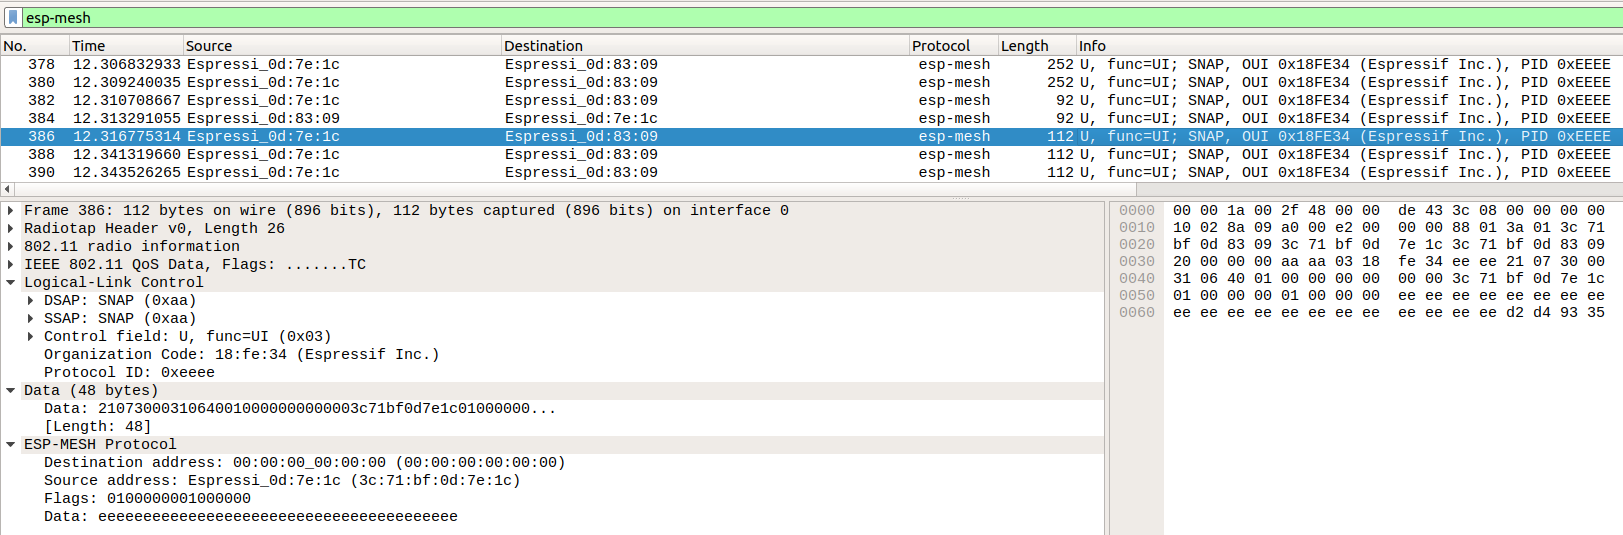
\includegraphics[scale=0.35]{images/wireSharkDissector.png}
            \caption{bla}
            \label{result_wiresharkDissector}
        \end{figure}
        
    %\end{enumerate}

    \section{ESP-NOW}
        Le driver Wi-Fi d'\textit{IDF} ne nous permet pas d'avoir une connexion avec plusieurs noeuds simultanément. 
        Nous supposons que c'est pour cette raison qu'\espmesh\ utilise une structure d'arbre et non de graphe.
        \espnow\ est une solution qui palie à ce problème.
        En effet un noeud peut avoir maximum 20 voisins. Ce qui est suffisant pour établir un réseau \mesh\ tel
        que nous l'envisagons. Par contre, comparé à \espmesh, le \textsc{mtu} est plus petit. En effet il est
        de 250 octets.\footnote{le \textsc{mtu} et le nombre de voisins maximum sont définis dans le fichier
        \textbf{esp\_now.h}}

        Utilisons \espnow:\\
        Nous avons utilisés 3 noeuds. Un des noeuds envoie des données en broadcast aux autres.
        Voici un exrait du code permettant de réalisé ce que nous venons de décrire:
        \begin{minted}[xleftmargin=\parindent,linenos]{c}

#define ESPNOW_WIFI_MODE WIFI_MODE_STA // Wi-Fi mode: sta, ap or sta+ap
#define ESPNOW_WIFI_IF ESP_IF_WIFI_STA // Wi-Fi interface sta or ap
static const uint8_t broadcast_addr[ESP_NOW_ETH_ALEN] = 
    {0xFF, 0xFF, 0xFF, 0xFF, 0xFF, 0xFF};
void espnow_recv_cb(const uint8_t *mac_addr, const uint8_t *data,
    int data_len){
    ESP_LOGI(TAG, "receive %d bytes:", data_len);
    printArray(data, data_len);
}
void esp_now_tx(void *arg){
    /* ... */
    esp_now_peer_info_t peer;//create peer broadcast
    peer.channel = CHANNEL;
    peer.ifidx = ESPNOW_WIFI_IF;
    peer.encrypt = false;
    memcpy(peer.peer_addr, broadcast_addr, ESP_NOW_ETH_ALEN);
    ESP_ERROR_CHECK(esp_now_add_peer(&peer)); // add peer
    while(is_running){
        esp_now_send(&broadcast_addr, &data, sizeof(data));
        vTaskDelay( 1000 / portTICK_PERIOD_MS ); // delay the task
    }
    vTaskDelete(NULL); 
}
void app_main(void){    
    /* ... */
    /* Wi-Fi initialization */
    wifi_init_config_t config = WIFI_INIT_CONFIG_DEFAULT();
    ESP_ERROR_CHECK(esp_wifi_init(&config));
    ESP_ERROR_CHECK(esp_wifi_set_mode(ESPNOW_WIFI_MODE));
    ESP_ERROR_CHECK(esp_wifi_start());
    /* ESP-NOW initialization */
    ESP_ERROR_CHECK(esp_now_init());
    ESP_ERROR_CHECK(esp_now_register_recv_cb(espnow_recv_cb));
    /* ... */
}
        \end{minted}
Tout d'abord nous initialisons le driver \wifi\ et nous définissions le mode du driver \wifi\ à
\textit{station}. Cette interface sera utilisée par \espnow. Il est également possible d'utiliser 
l'interface \textit{acces point}. 
Ensuite nous définissions la fonction qui sera appellée lorsqu'un paquet \espnow\ est reçu.
Après, nous créons, pour le noeud source, la tâche \textbf{esp\_now\_tx()} qui envoie les données en broadcast.
Pour cela, nous devons d'abord créer un "voisin" broadcast, pour ensuite envoyer les données vers ce voisin.
Pour envoyer des données vers un noeud précis, il faut créer un voisin avec l'adresse \mac\ du noeud.

Pour construire un réseau \mesh, il faudrait, par exemple que chaque nouveau noeud émette en broadcast, un paquet \espnow\ 
contenant au moins son adresse \mac. De cette façons, les noeuds voisins pourraient le rajouter à leurs
liste de voisins.